\documentclass[twoside]{book}

% Packages required by doxygen
\usepackage{fixltx2e}
\usepackage{calc}
\usepackage{doxygen}
\usepackage[export]{adjustbox} % also loads graphicx
\usepackage{graphicx}
\usepackage[utf8]{inputenc}
\usepackage{makeidx}
\usepackage{multicol}
\usepackage{multirow}
\PassOptionsToPackage{warn}{textcomp}
\usepackage{textcomp}
\usepackage[nointegrals]{wasysym}
\usepackage[table]{xcolor}

% Font selection
\usepackage[T1]{fontenc}
\usepackage[scaled=.90]{helvet}
\usepackage{courier}
\usepackage{amssymb}
\usepackage{sectsty}
\renewcommand{\familydefault}{\sfdefault}
\allsectionsfont{%
  \fontseries{bc}\selectfont%
  \color{darkgray}%
}
\renewcommand{\DoxyLabelFont}{%
  \fontseries{bc}\selectfont%
  \color{darkgray}%
}
\newcommand{\+}{\discretionary{\mbox{\scriptsize$\hookleftarrow$}}{}{}}

% Page & text layout
\usepackage{geometry}
\geometry{%
  a4paper,%
  top=2.5cm,%
  bottom=2.5cm,%
  left=2.5cm,%
  right=2.5cm%
}
\tolerance=750
\hfuzz=15pt
\hbadness=750
\setlength{\emergencystretch}{15pt}
\setlength{\parindent}{0cm}
\setlength{\parskip}{0.2cm}
\makeatletter
\renewcommand{\paragraph}{%
  \@startsection{paragraph}{4}{0ex}{-1.0ex}{1.0ex}{%
    \normalfont\normalsize\bfseries\SS@parafont%
  }%
}
\renewcommand{\subparagraph}{%
  \@startsection{subparagraph}{5}{0ex}{-1.0ex}{1.0ex}{%
    \normalfont\normalsize\bfseries\SS@subparafont%
  }%
}
\makeatother

% Headers & footers
\usepackage{fancyhdr}
\pagestyle{fancyplain}
\fancyhead[LE]{\fancyplain{}{\bfseries\thepage}}
\fancyhead[CE]{\fancyplain{}{}}
\fancyhead[RE]{\fancyplain{}{\bfseries\leftmark}}
\fancyhead[LO]{\fancyplain{}{\bfseries\rightmark}}
\fancyhead[CO]{\fancyplain{}{}}
\fancyhead[RO]{\fancyplain{}{\bfseries\thepage}}
\fancyfoot[LE]{\fancyplain{}{}}
\fancyfoot[CE]{\fancyplain{}{}}
\fancyfoot[RE]{\fancyplain{}{\bfseries\scriptsize Generated on Wed May 25 2016 18\+:13\+:06 for Bebop\+Piloting\+New\+A\+P\+I by Doxygen }}
\fancyfoot[LO]{\fancyplain{}{\bfseries\scriptsize Generated on Wed May 25 2016 18\+:13\+:06 for Bebop\+Piloting\+New\+A\+P\+I by Doxygen }}
\fancyfoot[CO]{\fancyplain{}{}}
\fancyfoot[RO]{\fancyplain{}{}}
\renewcommand{\footrulewidth}{0.4pt}
\renewcommand{\chaptermark}[1]{%
  \markboth{#1}{}%
}
\renewcommand{\sectionmark}[1]{%
  \markright{\thesection\ #1}%
}

% Indices & bibliography
\usepackage{natbib}
\usepackage[titles]{tocloft}
\setcounter{tocdepth}{3}
\setcounter{secnumdepth}{5}
\makeindex

% Hyperlinks (required, but should be loaded last)
\usepackage{ifpdf}
\ifpdf
  \usepackage[pdftex,pagebackref=true]{hyperref}
\else
  \usepackage[ps2pdf,pagebackref=true]{hyperref}
\fi
\hypersetup{%
  colorlinks=true,%
  linkcolor=blue,%
  citecolor=blue,%
  unicode%
}

% Custom commands
\newcommand{\clearemptydoublepage}{%
  \newpage{\pagestyle{empty}\cleardoublepage}%
}


%===== C O N T E N T S =====

\begin{document}

% Titlepage & ToC
\hypersetup{pageanchor=false,
             bookmarks=true,
             bookmarksnumbered=true,
             pdfencoding=unicode
            }
\pagenumbering{roman}
\begin{titlepage}
\vspace*{7cm}
\begin{center}%
{\Large Bebop\+Piloting\+New\+A\+P\+I }\\
\vspace*{1cm}
{\large Generated by Doxygen 1.8.9.1}\\
\vspace*{0.5cm}
{\small Wed May 25 2016 18:13:06}\\
\end{center}
\end{titlepage}
\clearemptydoublepage
\tableofcontents
\clearemptydoublepage
\pagenumbering{arabic}
\hypersetup{pageanchor=true}

%--- Begin generated contents ---
\chapter{R\+E\+A\+D\+M\+E}
\label{md_README}
\hypertarget{md_README}{}
This sample shows how to receive video stream from a Bebop Drone, decode it, display the decoded stream with mplayer and get inputs from users to control the Bebop drone.

\section*{To compile S\+D\+K Example Bebop\+Drone\+Decode\+Stream }

On Linux and Mac\+O\+S X platform \+: make

\section*{Dependencies of Bebop\+Drone\+Decode\+Stream }

You will need {\bfseries mplayer} to show the video stream, {\bfseries ffmpeg} to get the video decoded and {\bfseries ncurse} to get inputs from console

On Linux you can get ncurses-\/dev apt-\/get\+: apt-\/get install ncurses-\/dev

\section*{To run S\+D\+K Example Bebop\+Drone\+Decode\+Stream }

On Linux and Mac\+O\+S X platform \+: make run

\section*{To clean the compilation of Bebop\+Drone\+Decode\+Stream }

On Linux and Mac\+O\+S X platform \+: make clean

\section*{Discussion about Bebop\+Drone\+Decode\+Stream }

This project is separated into 3 classes \+:


\begin{DoxyItemize}
\item Bebop\+Drone\+Decode\+Stream \+: This is the main class. It will operate the connexion to the drone, the setup of the network and video part. It will also register for commands callback and send commands. If you need to add callbacks, add it in register\+A\+R\+Commands\+Callbacks.
\end{DoxyItemize}

In this class, the callback for a new frame received will be called. When it does, it will take a free empty frame from a pool (to avoid an allocation each time a frame is received), put the received data in this free frame and add the free frame to a frame buffer. An other thread will loop, and try to take a frame and pass it to the decoder. Once the frame has been decoded, it will write the decoded frame in a pipe file. M\+Player will read this pipe file and display the frames.


\begin{DoxyItemize}
\item Decoder\+Manager This is an util class that will perform h264 frame decoding thanks to ffmpeg.
\item ihm This is an util class that will catch inputs from console and send these events to Bebop\+Drone\+Decode\+Stream. It will also display some pieces of information about the drone, like its battery level and its flying state.
\end{DoxyItemize}

When you run this sample, be sure to be in the console to catch your keyboard event. As M\+Player will open a new window, you could have to click again in the console. The ihm inputs are implemented on an azerty keyboard. Feel free to adapt it just by changing the key comparison in the function I\+H\+M\+\_\+\+Input\+Processing. 
\chapter{Class Index}
\section{Class List}
Here are the classes, structs, unions and interfaces with brief descriptions\+:\begin{DoxyCompactList}
\item\contentsline{section}{\hyperlink{structIHM__t}{I\+H\+M\+\_\+t} }{\pageref{structIHM__t}}{}
\end{DoxyCompactList}

\chapter{File Index}
\section{File List}
Here is a list of all documented files with brief descriptions\+:\begin{DoxyCompactList}
\item\contentsline{section}{\hyperlink{BebopPiloting_8c}{Bebop\+Piloting.\+c} \\*This file contains sources about basic arsdk example sending commands to a bebop drone for piloting it and make it jump it and receiving its battery level }{\pageref{BebopPiloting_8c}}{}
\item\contentsline{section}{{\bfseries Bebop\+Piloting.\+h} }{\pageref{BebopPiloting_8h}}{}
\item\contentsline{section}{\hyperlink{ihm_8c}{ihm.\+c} \\*This file contains sources about ncurses I\+H\+M used by arsdk example \char`\"{}\+Jumping\+Sumo\+Piloting\char`\"{} }{\pageref{ihm_8c}}{}
\item\contentsline{section}{{\bfseries ihm.\+h} }{\pageref{ihm_8h}}{}
\end{DoxyCompactList}

\chapter{Class Documentation}
\hypertarget{structIHM__t}{}\section{I\+H\+M\+\_\+t Struct Reference}
\label{structIHM__t}\index{I\+H\+M\+\_\+t@{I\+H\+M\+\_\+t}}
\subsection*{Public Attributes}
\begin{DoxyCompactItemize}
\item 
\hypertarget{structIHM__t_a054e97c316934e2c096851218b77eeb0}{}W\+I\+N\+D\+O\+W $\ast$ {\bfseries main\+Window}\label{structIHM__t_a054e97c316934e2c096851218b77eeb0}

\item 
\hypertarget{structIHM__t_a26a01f7024501c6f6cb265a3ec63b51d}{}A\+R\+S\+A\+L\+\_\+\+Thread\+\_\+t {\bfseries input\+Thread}\label{structIHM__t_a26a01f7024501c6f6cb265a3ec63b51d}

\item 
\hypertarget{structIHM__t_a55f137fec8f1a4c6e7f750e867c5f572}{}int {\bfseries run}\label{structIHM__t_a55f137fec8f1a4c6e7f750e867c5f572}

\item 
\hypertarget{structIHM__t_a02dfaefc359fb07336c9489fd8218430}{}I\+H\+M\+\_\+on\+Input\+Event\+\_\+t {\bfseries on\+Input\+Event\+Callback}\label{structIHM__t_a02dfaefc359fb07336c9489fd8218430}

\item 
\hypertarget{structIHM__t_a7c9f6f8a2f01a3418c4690708b8cb910}{}void $\ast$ {\bfseries custom\+Data}\label{structIHM__t_a7c9f6f8a2f01a3418c4690708b8cb910}

\end{DoxyCompactItemize}


The documentation for this struct was generated from the following file\+:\begin{DoxyCompactItemize}
\item 
ihm.\+h\end{DoxyCompactItemize}

\chapter{File Documentation}
\hypertarget{BebopPiloting_8c}{}\section{Bebop\+Piloting.\+c File Reference}
\label{BebopPiloting_8c}\index{Bebop\+Piloting.\+c@{Bebop\+Piloting.\+c}}


This file contains sources about basic arsdk example sending commands to a bebop drone for piloting it and make it jump it and receiving its battery level.  


{\ttfamily \#include $<$stdlib.\+h$>$}\\*
{\ttfamily \#include $<$curses.\+h$>$}\\*
{\ttfamily \#include $<$string.\+h$>$}\\*
{\ttfamily \#include $<$unistd.\+h$>$}\\*
{\ttfamily \#include $<$signal.\+h$>$}\\*
{\ttfamily \#include $<$errno.\+h$>$}\\*
{\ttfamily \#include $<$lib\+A\+R\+S\+A\+L/\+A\+R\+S\+A\+L.\+h$>$}\\*
{\ttfamily \#include $<$lib\+A\+R\+Controller/\+A\+R\+Controller.\+h$>$}\\*
{\ttfamily \#include $<$lib\+A\+R\+Discovery/\+A\+R\+Discovery.\+h$>$}\\*
{\ttfamily \#include \char`\"{}Bebop\+Piloting.\+h\char`\"{}}\\*
{\ttfamily \#include \char`\"{}ihm.\+h\char`\"{}}\\*
Include dependency graph for Bebop\+Piloting.\+c\+:
\nopagebreak
\begin{figure}[H]
\begin{center}
\leavevmode
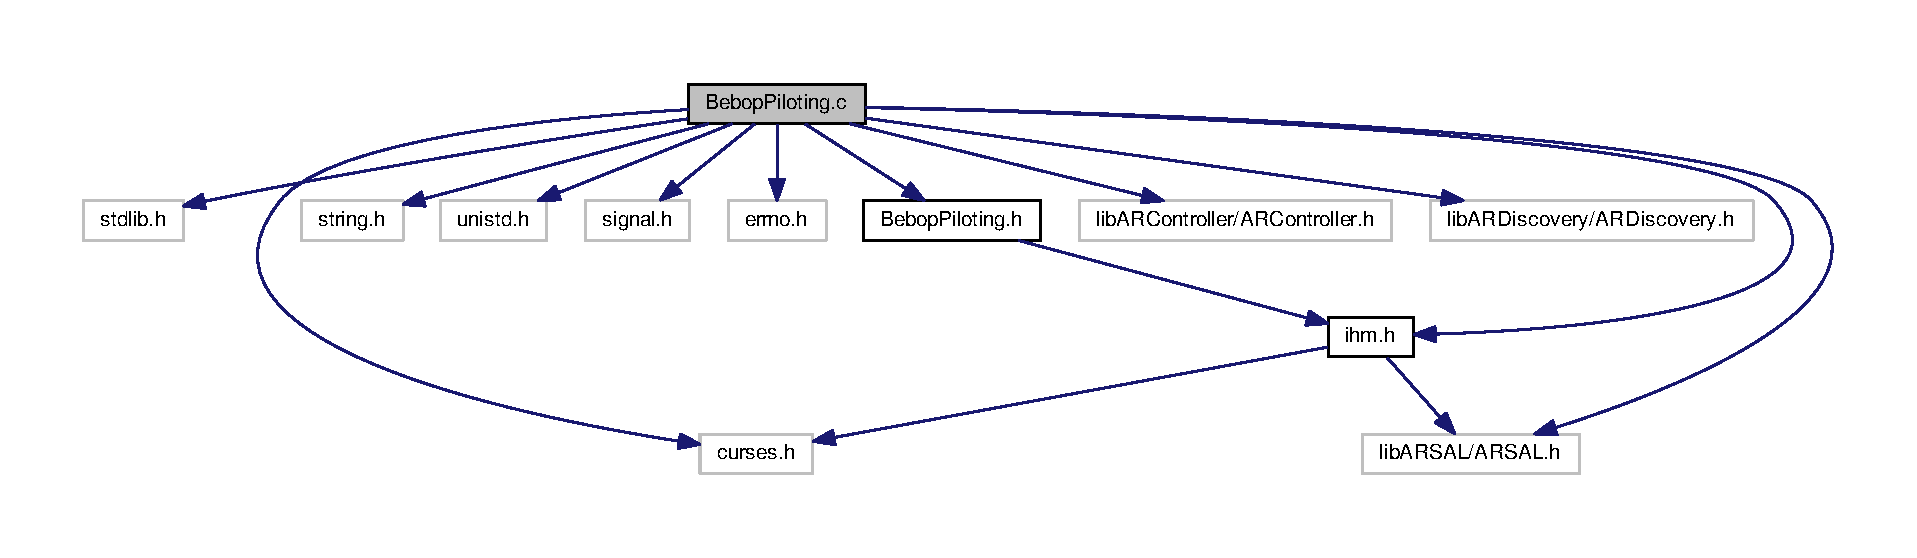
\includegraphics[width=350pt]{BebopPiloting_8c__incl}
\end{center}
\end{figure}
\subsection*{Macros}
\begin{DoxyCompactItemize}
\item 
\hypertarget{BebopPiloting_8c_afc3d101f633a076cc1ca84b85b6224b2}{}\#define {\bfseries T\+A\+G}~\char`\"{}S\+D\+K\+Example\char`\"{}\label{BebopPiloting_8c_afc3d101f633a076cc1ca84b85b6224b2}

\item 
\hypertarget{BebopPiloting_8c_a2411ca45269a59691454ca7c3b0f34f5}{}\#define {\bfseries E\+R\+R\+O\+R\+\_\+\+S\+T\+R\+\_\+\+L\+E\+N\+G\+T\+H}~2048\label{BebopPiloting_8c_a2411ca45269a59691454ca7c3b0f34f5}

\item 
\hypertarget{BebopPiloting_8c_acd0cd12adc95b2e0cec50f4374b32dff}{}\#define {\bfseries B\+E\+B\+O\+P\+\_\+\+I\+P\+\_\+\+A\+D\+D\+R\+E\+S\+S}~\char`\"{}192.\+168.\+42.\+1\char`\"{}\label{BebopPiloting_8c_acd0cd12adc95b2e0cec50f4374b32dff}

\item 
\hypertarget{BebopPiloting_8c_a3ab53ceedcb0afddba4c461f245e4cd7}{}\#define {\bfseries B\+E\+B\+O\+P\+\_\+\+D\+I\+S\+C\+O\+V\+E\+R\+Y\+\_\+\+P\+O\+R\+T}~44444\label{BebopPiloting_8c_a3ab53ceedcb0afddba4c461f245e4cd7}

\item 
\hypertarget{BebopPiloting_8c_a0fd24e9c1fd0f7fddb54b8167064d4ea}{}\#define {\bfseries D\+I\+S\+P\+L\+A\+Y\+\_\+\+W\+I\+T\+H\+\_\+\+M\+P\+L\+A\+Y\+E\+R}~1\label{BebopPiloting_8c_a0fd24e9c1fd0f7fddb54b8167064d4ea}

\item 
\hypertarget{BebopPiloting_8c_abc7fca69f0408724458bfe224397ad9c}{}\#define {\bfseries F\+I\+F\+O\+\_\+\+D\+I\+R\+\_\+\+P\+A\+T\+T\+E\+R\+N}~\char`\"{}/tmp/arsdk\+\_\+\+X\+X\+X\+X\+X\+X\char`\"{}\label{BebopPiloting_8c_abc7fca69f0408724458bfe224397ad9c}

\item 
\hypertarget{BebopPiloting_8c_a4e0d0f1b9bc23052255969da4c5ee560}{}\#define {\bfseries F\+I\+F\+O\+\_\+\+N\+A\+M\+E}~\char`\"{}arsdk\+\_\+fifo\char`\"{}\label{BebopPiloting_8c_a4e0d0f1b9bc23052255969da4c5ee560}

\item 
\hypertarget{BebopPiloting_8c_ae66af21320118d87b0d554b56b5eb5ea}{}\#define {\bfseries I\+H\+M}\label{BebopPiloting_8c_ae66af21320118d87b0d554b56b5eb5ea}

\end{DoxyCompactItemize}
\subsection*{Functions}
\begin{DoxyCompactItemize}
\item 
\hypertarget{BebopPiloting_8c_a0ddf1224851353fc92bfbff6f499fa97}{}int {\bfseries main} (int argc, char $\ast$argv\mbox{[}$\,$\mbox{]})\label{BebopPiloting_8c_a0ddf1224851353fc92bfbff6f499fa97}

\item 
\hypertarget{BebopPiloting_8c_acd97b9021b0a99c1a838fcdc1ed142b7}{}void {\bfseries state\+Changed} (e\+A\+R\+C\+O\+N\+T\+R\+O\+L\+L\+E\+R\+\_\+\+D\+E\+V\+I\+C\+E\+\_\+\+S\+T\+A\+T\+E new\+State, e\+A\+R\+C\+O\+N\+T\+R\+O\+L\+L\+E\+R\+\_\+\+E\+R\+R\+O\+R error, void $\ast$custom\+Data)\label{BebopPiloting_8c_acd97b9021b0a99c1a838fcdc1ed142b7}

\item 
\hypertarget{BebopPiloting_8c_a793e92c275c560533e5df6af59c92200}{}void {\bfseries command\+Received} (e\+A\+R\+C\+O\+N\+T\+R\+O\+L\+L\+E\+R\+\_\+\+D\+I\+C\+T\+I\+O\+N\+A\+R\+Y\+\_\+\+K\+E\+Y command\+Key, A\+R\+C\+O\+N\+T\+R\+O\+L\+L\+E\+R\+\_\+\+D\+I\+C\+T\+I\+O\+N\+A\+R\+Y\+\_\+\+E\+L\+E\+M\+E\+N\+T\+\_\+t $\ast$element\+Dictionary, void $\ast$custom\+Data)\label{BebopPiloting_8c_a793e92c275c560533e5df6af59c92200}

\item 
\hypertarget{BebopPiloting_8c_a70add123ba114ad9de1996a8b53cf939}{}void {\bfseries battery\+State\+Changed} (uint8\+\_\+t percent)\label{BebopPiloting_8c_a70add123ba114ad9de1996a8b53cf939}

\item 
\hypertarget{BebopPiloting_8c_a67670dff98b1ef27e30547e54cce7bfd}{}e\+A\+R\+C\+O\+N\+T\+R\+O\+L\+L\+E\+R\+\_\+\+E\+R\+R\+O\+R {\bfseries decoder\+Config\+Callback} (A\+R\+C\+O\+N\+T\+R\+O\+L\+L\+E\+R\+\_\+\+Stream\+\_\+\+Codec\+\_\+t codec, void $\ast$custom\+Data)\label{BebopPiloting_8c_a67670dff98b1ef27e30547e54cce7bfd}

\item 
\hypertarget{BebopPiloting_8c_a7c8d10c46f7c25da2a430f29ebd340ee}{}e\+A\+R\+C\+O\+N\+T\+R\+O\+L\+L\+E\+R\+\_\+\+E\+R\+R\+O\+R {\bfseries did\+Receive\+Frame\+Callback} (A\+R\+C\+O\+N\+T\+R\+O\+L\+L\+E\+R\+\_\+\+Frame\+\_\+t $\ast$frame, void $\ast$custom\+Data)\label{BebopPiloting_8c_a7c8d10c46f7c25da2a430f29ebd340ee}

\item 
\hypertarget{BebopPiloting_8c_a3bcbfca6eea9b5388a9ccbe000598e71}{}void {\bfseries on\+Input\+Event} (e\+I\+H\+M\+\_\+\+I\+N\+P\+U\+T\+\_\+\+E\+V\+E\+N\+T event, void $\ast$custom\+Data)\label{BebopPiloting_8c_a3bcbfca6eea9b5388a9ccbe000598e71}

\item 
\hypertarget{BebopPiloting_8c_aaebc87fd1d07a699d3b9f1ebd0791896}{}int {\bfseries custom\+Print\+Callback} (e\+A\+R\+S\+A\+L\+\_\+\+P\+R\+I\+N\+T\+\_\+\+L\+E\+V\+E\+L level, const char $\ast$tag, const char $\ast$format, va\+\_\+list va)\label{BebopPiloting_8c_aaebc87fd1d07a699d3b9f1ebd0791896}

\end{DoxyCompactItemize}
\subsection*{Variables}
\begin{DoxyCompactItemize}
\item 
\hypertarget{BebopPiloting_8c_a7d2ca1ba0336e57f2500231a6ca05091}{}int {\bfseries g\+I\+H\+M\+Run} = 1\label{BebopPiloting_8c_a7d2ca1ba0336e57f2500231a6ca05091}

\item 
\hypertarget{BebopPiloting_8c_a1f61d9e9cc96aa362c377e65aa9e408e}{}char {\bfseries g\+Error\+Str} \mbox{[}E\+R\+R\+O\+R\+\_\+\+S\+T\+R\+\_\+\+L\+E\+N\+G\+T\+H\mbox{]}\label{BebopPiloting_8c_a1f61d9e9cc96aa362c377e65aa9e408e}

\item 
\hypertarget{BebopPiloting_8c_a55486e11f62a946ac5023de669e7ba94}{}\hyperlink{structIHM__t}{I\+H\+M\+\_\+t} $\ast$ {\bfseries ihm} = N\+U\+L\+L\label{BebopPiloting_8c_a55486e11f62a946ac5023de669e7ba94}

\item 
\hypertarget{BebopPiloting_8c_ad223a59d932bdcba53172d117f456b74}{}F\+I\+L\+E $\ast$ {\bfseries video\+Out} = N\+U\+L\+L\label{BebopPiloting_8c_ad223a59d932bdcba53172d117f456b74}

\item 
\hypertarget{BebopPiloting_8c_a5296c5701714e4539efa1765c86c08bf}{}int {\bfseries frame\+Nb} = 0\label{BebopPiloting_8c_a5296c5701714e4539efa1765c86c08bf}

\item 
\hypertarget{BebopPiloting_8c_a587ffc7c6d0a6899d0aa91fb1fc0a7e1}{}A\+R\+S\+A\+L\+\_\+\+Sem\+\_\+t {\bfseries state\+Sem}\label{BebopPiloting_8c_a587ffc7c6d0a6899d0aa91fb1fc0a7e1}

\item 
\hypertarget{BebopPiloting_8c_a82537c84dc30bbc98714abd7741107fe}{}int {\bfseries is\+Bebop2} = 0\label{BebopPiloting_8c_a82537c84dc30bbc98714abd7741107fe}

\end{DoxyCompactItemize}


\subsection{Detailed Description}
This file contains sources about basic arsdk example sending commands to a bebop drone for piloting it and make it jump it and receiving its battery level. 

\begin{DoxyDate}{Date}
15/01/2015 
\end{DoxyDate}

\hypertarget{ihm_8c}{}\section{ihm.\+c File Reference}
\label{ihm_8c}\index{ihm.\+c@{ihm.\+c}}


This file contains sources about ncurses I\+H\+M used by arsdk example \char`\"{}\+Bebop\+Drone\+Decode\+Stream\char`\"{}.  


{\ttfamily \#include $<$stdlib.\+h$>$}\\*
{\ttfamily \#include $<$curses.\+h$>$}\\*
{\ttfamily \#include $<$string.\+h$>$}\\*
{\ttfamily \#include $<$lib\+A\+R\+S\+A\+L/\+A\+R\+S\+A\+L.\+h$>$}\\*
{\ttfamily \#include \char`\"{}ihm.\+h\char`\"{}}\\*
Include dependency graph for ihm.\+c\+:
\nopagebreak
\begin{figure}[H]
\begin{center}
\leavevmode
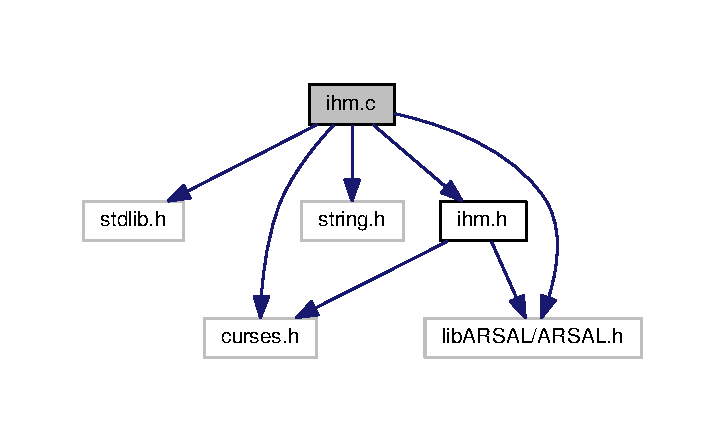
\includegraphics[width=348pt]{ihm_8c__incl}
\end{center}
\end{figure}
\subsection*{Macros}
\begin{DoxyCompactItemize}
\item 
\hypertarget{ihm_8c_a58017ec045269446009126ad5f844356}{}\#define {\bfseries H\+E\+A\+D\+E\+R\+\_\+\+X}~0\label{ihm_8c_a58017ec045269446009126ad5f844356}

\item 
\hypertarget{ihm_8c_add11cdd656672eaeef4410dda5937b0d}{}\#define {\bfseries H\+E\+A\+D\+E\+R\+\_\+\+Y}~0\label{ihm_8c_add11cdd656672eaeef4410dda5937b0d}

\item 
\hypertarget{ihm_8c_abe06bdb66452ea025f4ca3117856e54c}{}\#define {\bfseries I\+N\+S\+T\+R\+U\+C\+T\+I\+O\+N\+\_\+\+X}~0\label{ihm_8c_abe06bdb66452ea025f4ca3117856e54c}

\item 
\hypertarget{ihm_8c_a0661a392db40be1552f576a54f1c8c33}{}\#define {\bfseries I\+N\+S\+T\+R\+U\+C\+T\+I\+O\+N\+\_\+\+Y}~2\label{ihm_8c_a0661a392db40be1552f576a54f1c8c33}

\item 
\hypertarget{ihm_8c_a23cab0b49444cc4870f0d671f3d03ace}{}\#define {\bfseries B\+A\+T\+T\+E\+R\+Y\+\_\+\+X}~0\label{ihm_8c_a23cab0b49444cc4870f0d671f3d03ace}

\item 
\hypertarget{ihm_8c_a94ccb05dea98d7f090d5af6a7143eacb}{}\#define {\bfseries B\+A\+T\+T\+E\+R\+Y\+\_\+\+Y}~10\label{ihm_8c_a94ccb05dea98d7f090d5af6a7143eacb}

\item 
\hypertarget{ihm_8c_a741dafa1bd1ea79378f402bb15fbeeca}{}\#define {\bfseries I\+N\+F\+O\+\_\+\+X}~0\label{ihm_8c_a741dafa1bd1ea79378f402bb15fbeeca}

\item 
\hypertarget{ihm_8c_a89904cb639d01dbee42b37befc20650c}{}\#define {\bfseries I\+N\+F\+O\+\_\+\+Y}~12\label{ihm_8c_a89904cb639d01dbee42b37befc20650c}

\end{DoxyCompactItemize}
\subsection*{Functions}
\begin{DoxyCompactItemize}
\item 
\hypertarget{ihm_8c_a745d6e022c26b5c342d0c452be45daba}{}void $\ast$ {\bfseries I\+H\+M\+\_\+\+Input\+Processing} (void $\ast$data)\label{ihm_8c_a745d6e022c26b5c342d0c452be45daba}

\item 
\hypertarget{ihm_8c_a0c80596eb686749500f4f028f1b96e03}{}\hyperlink{structIHM__t}{I\+H\+M\+\_\+t} $\ast$ {\bfseries I\+H\+M\+\_\+\+New} (I\+H\+M\+\_\+on\+Input\+Event\+\_\+t on\+Input\+Event\+Callback)\label{ihm_8c_a0c80596eb686749500f4f028f1b96e03}

\item 
\hypertarget{ihm_8c_a16fdfbb07176c17e294bbd2aff53f36d}{}void {\bfseries I\+H\+M\+\_\+\+Delete} (\hyperlink{structIHM__t}{I\+H\+M\+\_\+t} $\ast$$\ast$ihm)\label{ihm_8c_a16fdfbb07176c17e294bbd2aff53f36d}

\item 
\hypertarget{ihm_8c_ae15b885587a1ad3ce40cd267a15d4ab9}{}void {\bfseries I\+H\+M\+\_\+set\+Custom\+Data} (\hyperlink{structIHM__t}{I\+H\+M\+\_\+t} $\ast$ihm, void $\ast$custom\+Data)\label{ihm_8c_ae15b885587a1ad3ce40cd267a15d4ab9}

\item 
\hypertarget{ihm_8c_a026e2b72ec609344806c307c4946fd07}{}void {\bfseries I\+H\+M\+\_\+\+Print\+Header} (\hyperlink{structIHM__t}{I\+H\+M\+\_\+t} $\ast$ihm, char $\ast$header\+Str)\label{ihm_8c_a026e2b72ec609344806c307c4946fd07}

\item 
\hypertarget{ihm_8c_a1b4881214982f377f9d7edcef574ff5f}{}void {\bfseries I\+H\+M\+\_\+\+Print\+Instruction} (\hyperlink{structIHM__t}{I\+H\+M\+\_\+t} $\ast$ihm, char $\ast$instruction\+Str)\label{ihm_8c_a1b4881214982f377f9d7edcef574ff5f}

\item 
\hypertarget{ihm_8c_ae9098136f2de628d2537fd84eba10b1e}{}void {\bfseries I\+H\+M\+\_\+\+Print\+Info} (\hyperlink{structIHM__t}{I\+H\+M\+\_\+t} $\ast$ihm, char $\ast$info\+Str)\label{ihm_8c_ae9098136f2de628d2537fd84eba10b1e}

\item 
\hypertarget{ihm_8c_af0d8adaf58223e18f35ea379ebeb5dbd}{}void {\bfseries I\+H\+M\+\_\+\+Print\+Battery} (\hyperlink{structIHM__t}{I\+H\+M\+\_\+t} $\ast$ihm, uint8\+\_\+t percent)\label{ihm_8c_af0d8adaf58223e18f35ea379ebeb5dbd}

\end{DoxyCompactItemize}


\subsection{Detailed Description}
This file contains sources about ncurses I\+H\+M used by arsdk example \char`\"{}\+Bebop\+Drone\+Decode\+Stream\char`\"{}. 

\begin{DoxyDate}{Date}
15/01/2015 
\end{DoxyDate}

%--- End generated contents ---

% Index
\backmatter
\newpage
\phantomsection
\clearemptydoublepage
\addcontentsline{toc}{chapter}{Index}
\printindex

\end{document}
